
\begin{NOTE}{ 例题 [洛谷 P4781 【模板】拉格朗日插值](https://www.luogu.org/problemnew/show/P4781)}{}

\end{NOTE}


\subsubsection{题目大意}

给出 $n$ 个点 $P_i(x_i,y_i)$ ,将过这 $n$ 个点的最多 $n-1$ 次的多项式记为 $f(x)$ ,求 $f(k)$ 的值。

\subsubsection{方法 1:差分法}

差分法适用于 $x_i=i$ 的情况。

如,用差分法求 $f(x)=\sum_{i=1}^{x} i^2$ 的多项式形式。

\vskip 0.2 in
\texttt{
1   5   14   30   55   91\\  4   9    16   25   36\\    5   7     9   11\\      2    2    2}
\vskip 0.2 in

第一行为 $f(x)$ 的连续的前几项;若上面一行有 $n$ 个值,下面一行有 $n-1$ 个值,每个值为上面对应的相邻两项的差。观察到,如果这样操作的次数足够多(前提是 $f(x)$ 为多项式),每次总会返回一个定值,可以利用这个定值求出 $f(x)$ 的每一项的系数,然后即可将 $k$ 代入多项式中求解。如上例中可求出 $f(x)=\frac 1 3 n^3+\frac 1 2 n^2+\frac 1 6 n$ 。时间复杂度为 $O(n^2)$ ,对给出的点的限制性较强。

\subsubsection{方法 2:高斯消元}

使用 \textbf{ 待定系数法 } 。设 $f(x)=\sum_{i=0}^{n-1} a_ix^i$将每个 $x_i$ 代入 $f(x)$ ,有 $f(x_i)=y_i$ ,这样就可以得到一个由 $n$ 条 $n$ 元 $1$ 次方程所组成的方程组,然后使用 \textbf{ 高斯消元 } 求出每一项 $a_i$ ,然后将 $k$ 代入求值。

如果您不知道什么是高斯消元,请看 \href{https://www.luogu.org/problemnew/show/P3389}{luogu P3389 高斯消元法} 。

时间复杂度 $O(n^3)$ ,对给出点的坐标无要求。

\subsubsection{方法 3: 拉格朗日差值法}

考虑将每个点做一个对于 $x$ 轴的垂线,设垂足为 $H_i(x_i,0)$ 。

\begin{figure}[h]
\centering
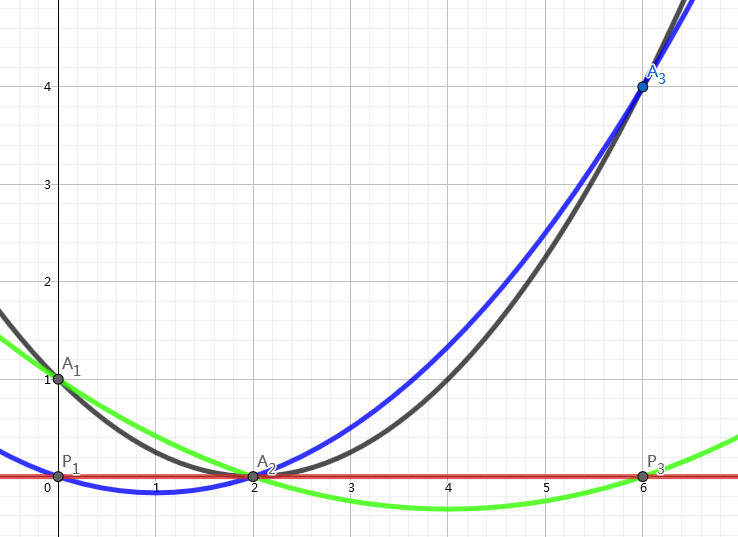
\includegraphics[width=0.5\textwidth]{images/lagrange-poly-1.png} 

\end{figure}

如上图所示,黑线等于蓝线加绿线加红线。每次我们选择 $1$ 个 $P_i$ ,并选择其他的 $H_j[j\neq i]$ ,做一条过这些点的一条至多 $n-1$ 次的线。由于有 $n-2$ 个点都在 $x$ 轴上,我们知道这条线的解析式一定是形如 $g_i(x)=y_i\times (\prod_{i=1}^{n} (x-x_i)[i\neq x])$ 的形式。

最后将所有的 $g(x)$ 相加,即 $f(x)=sum_{i=1}^{n}g_i(x)$ 。因为对于每个点 $P_i$ ,都只有一条函数经过 $P_i$ ,其余都经过 $H_i$ ,这一项的系数是 $0$ ,所以最后的和函数总是过所有 $n$ 个点的。

公式整理得:

$f(x)=\sum_{i=1}^{n} y_i\times(\prod_{j\neq i }\frac{x-x_j}{x_i-x_j})$

如果要将每一项都算出来,时间复杂度仍是 $O(n^2)$ 的,但是本题中只用求出 $f(k)$ 的值,所以只需将 $k$ 代入进式子里得:

$Ans=\sum_{i=1}^{n} y_i\times(\prod_{j\neq i }\frac{k-x_j}{x_i-x_j})$

本题中,还需要求解逆元。如果先分别计算出分子和分母,在计算分母的逆元,乘上分子,累加进最后的答案,时间复杂度的瓶颈就不会在求逆元上,时间复杂度为 $O(n^2)$ 。

\subsubsection{代码实现}

\begin{cppcode}
#include <algorithm>
#include <cstdio>
#include <cstring>
using namespace std;
const int maxn = 2010;
typedef long long ll;
ll mod = 998244353;
ll n, k, x[maxn], y[maxn], ans, s1, s2;
ll powmod(ll a, ll x) {
  ll ret = 1ll, nww = a;
  while (x) {
    if (x & 1) ret = ret * nww % mod;
    nww = nww * nww % mod;
    x >>= 1;
  }
  return ret;
}
ll inv(ll x) { return powmod(x, mod - 2); }
int main() {
  scanf("%lld%lld", &n, &k);
  for (int i = 1; i <= n; i++) scanf("%lld%lld", x + i, y + i);
  for (int i = 1; i <= n; i++) {
    s1 = y[i] % mod;
    s2 = 1ll;
    for (int j = 1; j <= n; j++)
      if (i != j)
        s1 = s1 * (k - x[j]) % mod, s2 = s2 * ((x[i] - x[j] % mod) % mod) % mod;
    ans += s1 * inv(s2) % mod;
    ans = (ans + mod) % mod;
  }
  printf("%lld\n", ans);
  return 0;
}
\end{cppcode}
